\section{Real World Smart Traffic}
In diesem Kapitel werden die Hintergründe für die Einführung von Smart-Traffic erläutert und welche Probleme dadurch bereits gelöst werden. Darüber hinaus werden Kritikpunkte erörtert sowie existierende Lösungen erläutert.

\subsection{Hintergrund -  Klima, Gesellschaft und Wirtschaft}

Die Umweltbelastungen durch Treibhausgase sind im vergangen Jahrhundert auf ein für unser Klima bedrohliches Maß angewachsen. In der Weltgesellschaft wird darüber besonders im Kontext der \emph{Erderwärmung} gesprochen. 1896 gelang dem schwedischen Nobelpreisträger Svante Arrhenius der mathematische Nachweis, dass eine Erhöhung der Treibhausgase zu einer Erhöhung der mittleren Erdtemperatur führt \citep[vgl.][]{SvanteArrhenius.1896}. Bei der internationalen geophysikalischen Konferenz 1957 wurden schließlich unwiderlegbare Beweise für die Erhöhung der Treibhausgase in der Atmosphäre geliefert \citep[vgl.][]{Rahmstorf.2007}. Die Auswirkungen der Erderwärmung sind seitdem vielseitig untersucht worden. Eine ausführliche Beschreibung anhand verschiedener Studien bietet das Forschungsinstitut \emph{Germanwatch}, welches vom Bundesamt für wirtschaftliche Zusammenarbeit und Entwicklung gefördert wird. Zusammengefasst lassen sich große und unkontrollierbare Gefahren für den Mensch, die Umwelt und das Ökosystem ableiten \citep{Rothenbucher.2011,Eis.2010}. Im Jahre 2002 hat die Europäische Union das Kyoto-Protokoll ratifiziert. Bis zum Jahr 2030 sollen sich die Treibhausgas -Emissionen um 40\% gegenüber dem Jahr 1990 verringern. Auf der Pariser Klimakonferenz 2015 haben sich 195 Staaten zum selben Ziel bekannt. Die globale Erwärmung soll auf ein Niveau von unter 2 Grad Celsius sinken, was dem vorindustriellen Niveau unserer Zeit entspricht. In Deutschland wurden die Ziele des Pariser Abkommens zum Leitbild für eine neue Klimaschutzpolitik. Daraus wurde der \emph{Klimaschutzplan 2050} erarbeitet, welcher eine Zieldefinition für bestimmt Handlungsfelder beinhaltet. In Abb. \ref{fig4} ist der Klimaschutzplan tabellarisch für die Etappe bis zum Jahr 2030 erfasst. Im Bereich Verkehr hat die Bundesregierung ein Einsparpotential zwischen 40-42\% kalkuliert. Im Frühjahr 2016 veröffentlichte das Kraftfahrtbundesamt eine Statistik zu den Treibhausgas-Emissionen in Deutschland von 1990 bis 2016 nach Kategorien der UNFCCC-Berichterstattung (Klimarahmenkonvention der Vereinten Nationen nach Pariser Abkommen). Insgesamt ist im Diagramm der Abbildung \ref{fig3} eine deutlich sichtbare Verringerung der Treibhaus-Emissionen zu beobachten. Vor allem in den Kategorien Energiewirtschaft und Industrieprozesse haben die Emissionen stark nachgelassen. Allerdings hat sich in der Kategorie Verkehr  kaum etwas verändert. Hier sind die Emissionen auf einem konstanten Niveau geblieben. 

\begin{figure}[ht]
	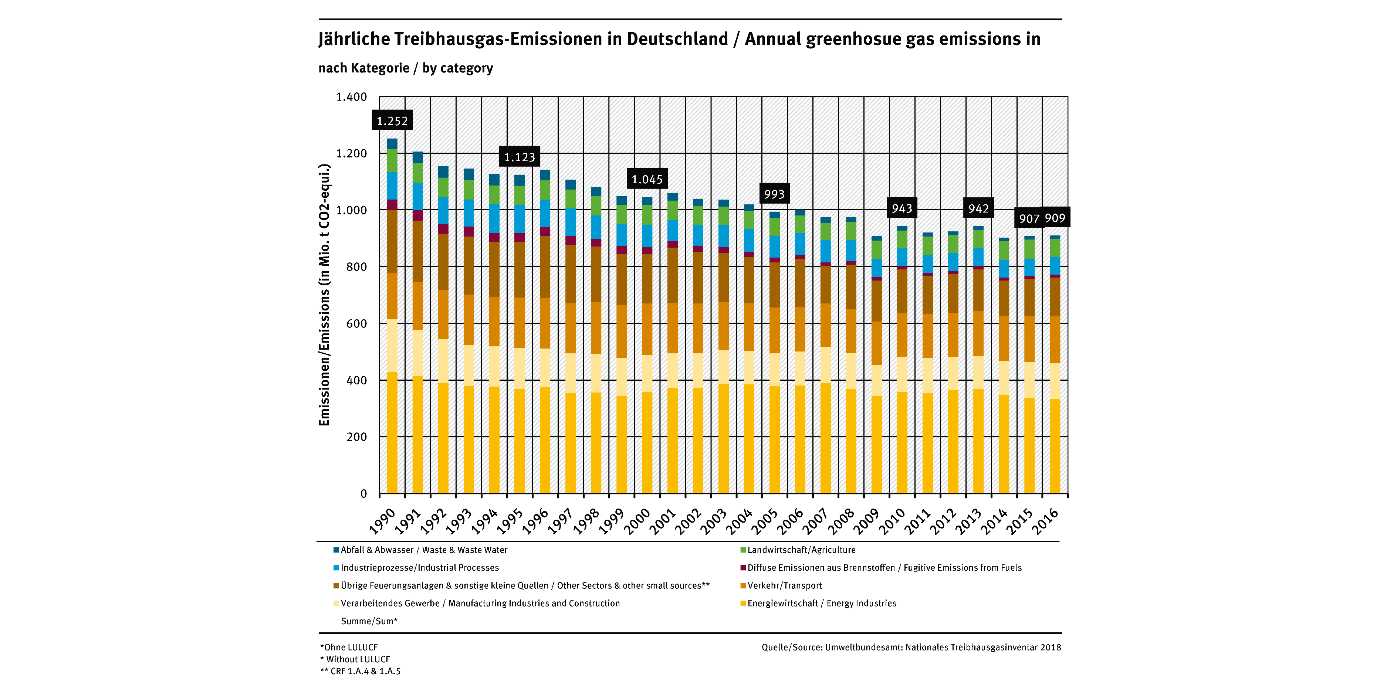
\includegraphics[width=\textwidth]{images/jaehrlicheTreibhausEmissionen.png}
	\caption{Entwicklung der jährlichen Treibhausemissionen in Deutschland}
	\label{fig3}
\end{figure}

Die Verbesserungen in den Bereichen Energiewirtschaft und Industrieprozesse lassen sich vor allem auf technologische Fortschritte zurückführen. Mit moderner Filter- und Anlagentechnik wurden effektive Maßnahmen durchgesetzt, um umweltfreundlicher beziehungsweise emissionsärmer zu produzieren. Im Verkehr hingegen hat der technische Fortschritt in der Fahrzeugbranche kaum einen Emissionsvorteil gebracht(siehe Abbildung …). Eine im Mai 2018 erschiene Statistik des Kraftfahrtbundesamtes lässt auf einen technologischen Fortschritt hinsichtlich Emissionen in der Automobilbranche schließen. So veränderte sich der durchschnittliche Kraftstoffverbrauch eines Automobils von 1995 bis 2016 von 8.8 Liter auf 7.2 Liter pro 100km \citep[vgl.][]{Umweltbundesamt.2018}. Abb.\ref{fig3} zeigt zudem die deutliche Verringerung der Emissionen von PKWs zwischen 1995 und 2014. Aufgrund des Anstiegs von 4,5 Millionen (1960) auf heute 46 Millionen gemeldeter Kraftfahrzeuge \citep[vgl.][]{StatistaDasStatistikPortal.2018}, hat sich der kumulierte Emissionsausstoß des Verkehrsektors, wie Abb. \ref verdeutlicht, nicht reduziert. Die Jahresbilanz des Kraftfahrtbundesamt weißt sogar 63,7 Millionen zugelassene Fahrzeuge aus \citep[vgl.][]{KBA.2018}. Die Umweltbelastung dieses Verkehrsaufkommen zeigt sich beispielsweise in der Region Stuttgart. Die Anzahl der sogenannten \emph{Feinstaubalarme} ist in den vergangenen Jahren kontinuierlich gestiegen. Von Oktober 2017 bis 2018 wurde der Alarmstatus an 56 Tagen ausgerufen. Hauptgrund ist, nach der Bilanz des Verkehrsministeriums Baden-Württemberg, der Straßenverkehr \citep[vgl.][]{MinisteriumfurVerkehrBadenWurttemberg.2018}.

\begin{figure}[ht]
	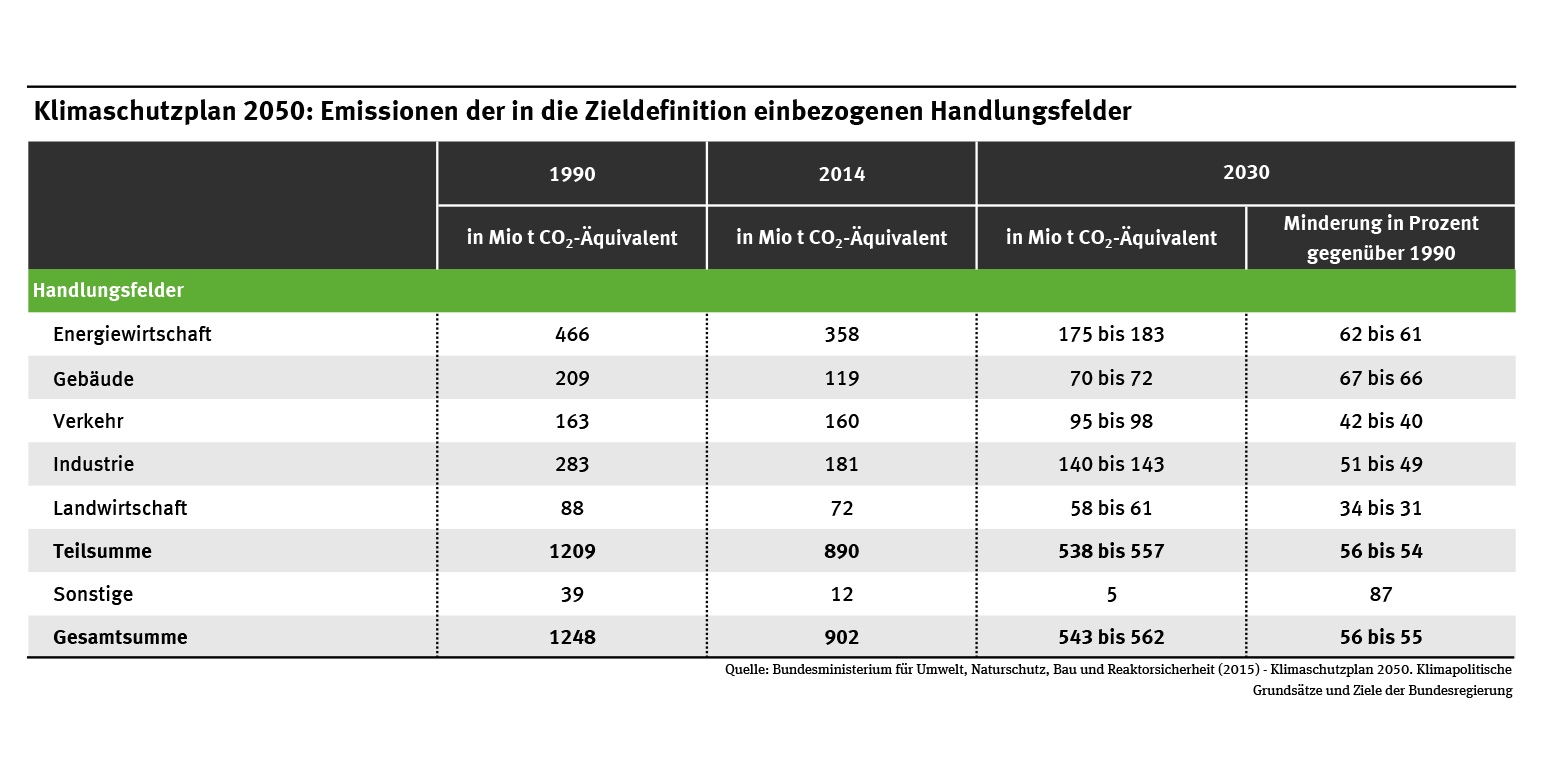
\includegraphics[width=\textwidth]{images/klimaschutzplan2050.png}
	\caption{Deutsche Ziele des Klimaschutzplans bis 2030}
	\label{fig4}
\end{figure}
%[QUELLE: https://www.umweltbundesamt.de/daten/klima/klimaschutzziele-deutschlands]

\begin{figure}[ht]
	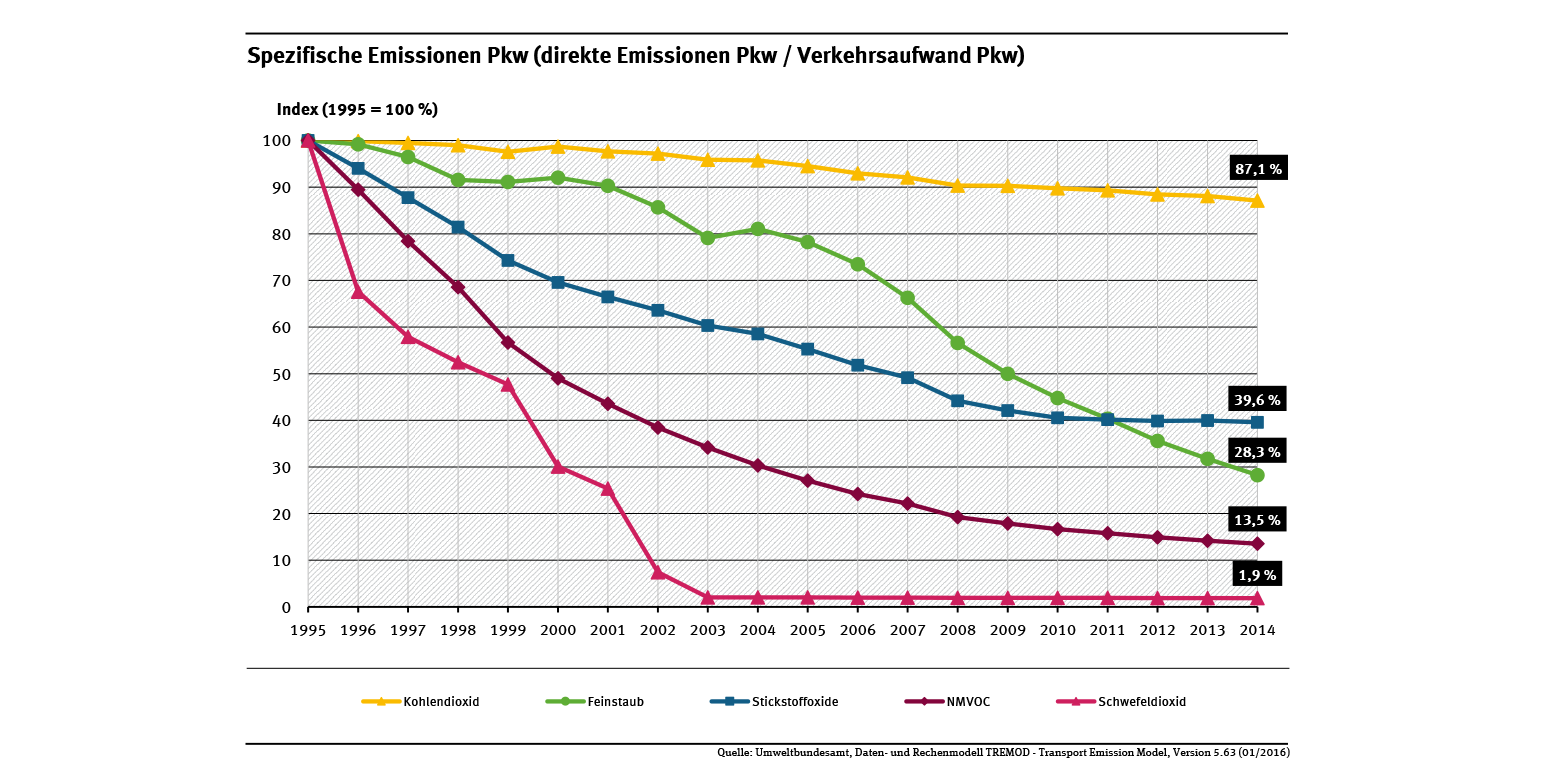
\includegraphics[width=\textwidth]{images/EntwicklungEmissionsentwicklungPKWs.png}
	\caption{Entwicklung der PKW-Emissionen}
	\label{fig12}
\end{figure}

Neben der Umweltbelastung führt die Verkehrslast zu weiteren signifikanten Problemen. Deutschlandweit gab es nach der ADAC Staubilanz im Jahr 2017 insgesamt 723000 Staus mit einer Gesamtlänge von knapp 1,5 Millionen Kilometer. Etwa 80\% der Staus fallen auf die Werktage von Montag bis Freitag und werden durch den Berufsverkehr beziehungsweise den ökonomischen Verkehr bedingt \citep[vgl.][]{ADAC.2018}. Somit wird aus dem Verkehrsaufkommen ein wesentlicher Wirtschaftsfaktor. Das Statistikinstitut \emph{INRIX} hat in Kooperation mit dem \emph{Centre of Economics and Business Research} die Kosten durch Verkehrsstaus prognostiziert. Kumuliert für das Zeitintervall zwischen 2013 bis 2030 ergibt sich in Deutschland ein ökonomisch wirksamer Schaden von 520 Milliarden Euro. Im Mittel entspricht das einem wirtschaftlichen Gesamtverlust von 33 Milliarden Euro pro Jahr und einer Belastung von über 2200 Euro pro individuellem Haushalt in Deutschland \citep[vgl.][]{INRIX.2014}. Bei der Betrachtung einzelner Individuen im Straßenverkehr kann die Auswirkung von Staus auf die menschliche Psyche analysiert werden. Laut der INRIX Studie stehen Verkehrsteilnehmer in den Ballungszentren im Schnitt 45 Stunden pro Jahr im Stau. Den Einfluss auf die menschliche Psyche wurde in einer vom Navigationssystemherstellers \emph{TomTom} in Auftrag gegebenen Studie ermittelt. Dafür wurden Probanden, welche länger im Stau standen, Speichelproben entnommen. In den Proben ließen sich sogenannte psychologische Stress-Marker feststellen, wodurch eine Aussage zum Stressniveau des Probanden möglich ist. Während bei weiblichen Probanden im Schnitt nur eine Erhöhung des Stressniveaus von 8,7\% festgestellt wurde, stieg das Stressniveau bei männlichen Probanden um 60\% \citep[vgl.][]{TomTom.2011}. 

\subsection{Smart Traffic Lösung}
%
%Im Kapitel Hintergrund – Klima, Gesellschaft, Wirtschaft wurden verschiedene Themen analysiert und Problemstellungen beschrieben, welche durch das faktisch bewiesene, zunehmende Verkehrsaufkommen entstehen. Zusammengefasst wurden die Einflüsse auf verschiedene Aspekte erörtert:
%\begin{itemize}
%\item Umweltbelastung
%\item Wirtschaft/Ökonomischer Schaden
%\item Gesellschaft/Psychischer Faktor der Verkehrsindividuen
%\end{itemize}

Wie kann nun die in Abb.\ref{fig4} dargestellten Zieldefinition der Klimakonvention erreicht werden?. Wie kann der negative ökonomischen Einfluss des Verkehrs verringert werden? Mit Hilfe von Smart Traffic wird versucht, den Problemen entgegen zu wirken. Abb.\ref{fig13} verdeutlicht, wie im Kontext von \emph{Big Data} der Smart Traffic Gesamtprozess alle Ansätze verbindet. Durch empirische Datenerhebungen zu Verkehrsszenarien lassen sich Muster herleiten, die beispielsweise auf einen Stau hindeuten oder eine erhöhte Umweltbelastung darstellen. Durch innovative Sensoren-Systeme können diese Muster in Echtzeit erkannt und Gegenmaßnahmen, wie zum Beispiel Umleitungen, angestoßen werden.
Ein flüssiger, effizienter Verkehrsstrom fördert eine Verminderung von unnötigem Kraftstoffverbrauch, was langfristig zur Reduzierung der Umweltbelastung beiträgt. Intelligente Straßenführung hat ein enormes Potential hinsichtlich Stauprävention, wodurch der negativ korrelierte Wirtschaftsfaktor minimiert werden kann. Zudem verringert sich die Zeit, welche Verkehrsteilnehmer in Staus verbringen. Vor allem in den Ballungszentren kann dies zu einer wesentlichen Verbesserung der allgemeinen Lebensqualität führen. Chancen und Perspektiven der Smart City und speziell die der innovativen Mobilitätsformen (Smart Traffic), wurden im Jahr 2017 von der renommierten Ratingagentur KMPG untersucht. In dem Report wird das Sparpotential durch ein effizienteres Management des Verkehrsaufkommens mit 60\% bewertet \citep[vgl.][]{KPMG.2017}. Smart Traffic Lösungen bieten also eine Vielzahl von Vorteilen, weshalb auf der ganzen Welt immer mehr Projekte und Realisierungen gestartet werden. Im Absatz \ref{smartTrafficGermany} werden einige Beispiele genannt.\\ 
Allerdings entstehen durch einfache Überlegungen auch einige Kritikpunkte am Smart Traffic Ansatz beziehungsweise in Bezug auf die Automatisierung des Verkehrsflusses und Lösungen durch detektierende Sensoren. 

\begin{figure}[ht]
\begin{center}
	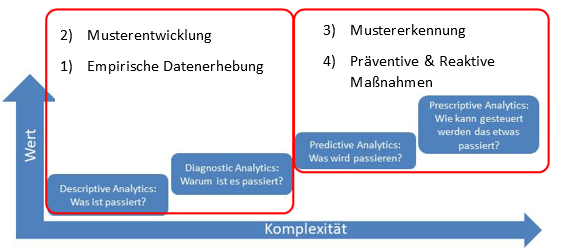
\includegraphics[scale=0.5]{images/SmartTrafficEinordnungBigDataThemengebiete.png}
	\caption{Smart Traffic Einordnung in BigData Themengebiete \citep[in Anlehnung an][]{RyoheiFujimaki.2016}}
	\label{fig13}
\end{center}

\end{figure}

\subsection{Smart Traffic Kritik}

Für den Ausbau der nötigen Infrastruktur eines Smart Traffic Systems muss ein großes Investitionsvolumen gestemmt werden. Zudem muss über den Datenschutz und rechtliche Themen diskutiert werden, denn Smart Traffic bietet dem Träger der Systeme diverse Überwachungs- und Kontrolloptionen. Außerdem muss die Frage der Verbindlichkeit beziehungsweise der Haftung für Unfälle in Folge der Fremdbestimmung durch Automatisierung geklärt werden. Kritisch muss auch die Gefahr der Digitalisierung betrachtet werden. Im Straßenverkehr sind überabzählbar unendlich viele Kombinationen von Verkehrsereignissen möglich, weshalb komplexe Realisierungen für die Mustererkennung und Maßnahmensteuerung digital mit Computern unterstützt werden müssen. Smart Traffic beschäftigt sich sozusagen mit der \emph{Steuerung} von Individuen, weshalb ein großes Sicherheitsniveau gegen Manipulation und Angreifbarkeit sichergestellt werden muss. Die Frage ist, ob die Absicherung der Systeme in einem geeigneten Maß überhaupt umgesetzt werden kann.\\
Unabhängig der offenen Fragen und Kritikpunkte, existieren weltweit funktionierende Ansätze für Smart Traffic. Welche Ansätze in Deutschland verfolgt werden, wird im nachfolgenden Abschnitt vorgestellt.

\subsection{Smart Traffic Projekte in Deutschland}\label{smartTrafficGermany}
Die hier vorgestellten Projekte sollen einen Überblick verschaffen, wie weit die Vernetzung des Straßenverkehrs in Deutschland bereits fortgeschritten ist.


\subsubsection{Sensorsystem Siemens Traffic Universal}
Siemens hat schon früh in die Entwicklung von Technologien investiert, die für die Anwendung in Smart Traffic Lösungen gedacht sind. Mit dem in Abb.\ref{fig14} dargestellten \textit{Siemens Traffic Eye} System lassen sich Daten, wie die Anzahl der Fahrzeuge, Geschwindigkeit, Verkehrsdichte und sogar die Klassifizierung der Fahrzeuge detektieren. Der größte Vorteil der Sensoren besteht darin, dass sie keine eigenständige Verkabelung benötigen. Die über Funk vernetzten Sensoren beziehen ihre Energie über Solarpanele. Das System ist vor allem in Berlin und im gesamten Ruhrgebiet verbreitet. Mit mehr als 3500 Installationen deutschlandweit ist Siemens derzeit einer der größten Vertreter auf dem Markt.

\begin{figure}[ht]
\begin{center}
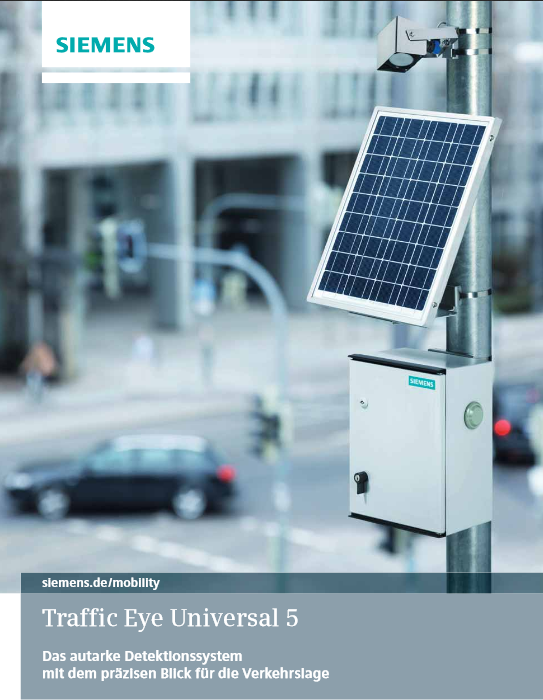
\includegraphics[scale=0.3]{images/SiemensTrafficEyeSensor.png}
	\caption{Siemens Traffic Eye Sensor}
	\label{fig14}
\end{center}

\end{figure}

\subsubsection{Parkleitsystem Park Here}
ParkHere ist eine sehr interessante Umsetzung für den Bereich Smart Traffic. Die Idee beruht im Grunde darauf Parkplätze mit Sensoren auszustatten, welche die Belegung an ein Zentralsystem kommunizieren. Nutzer der Mobilen App ParkHere können dann einsehen, welche Parkplätze derzeit zur Verfügung stehen. Da die Sensoren technologisch simpel sind und per Solarenergie betrieben werden, ist diese Lösung im Vergleich zu den umfangreicheren Smart Traffic Infrastrukturprojekten wirtschaftlich sehr rentabel. In München wird das System bereits eingesetzt. Zudem arbeitet das StartUp hinter der Idee inzwischen mit BMW an der Weiterentwicklung dieses Ansatzes.

\subsubsection{Smart Port Traffic}
\emph{Im Ha­fen Ham­burg ge­währ­leis­tet mo­derns­te di­gi­ta­le In­tel­li­genz ei­nen rei­bungs­lo­sen und ef­fi­zi­en­ten Be­trieb.} (Slogan der Hamburg Port Authority)\\
Für dieses Ziel werden in dem Gebiet verschiedene Sensoren genutzt, welche  Auskunft über die Auslastung der Straßenverbindungen in Echtzeit analysieren. Zudem sind LKWs mit RFID Chips ausgestattet um effiziente Transportwege zu gewährleisten. Unter dem Begriff Vehicle-to-X Kommunikation bezeichnet man die Verbindung zwischen RDIF Chips und Ampeln in der Zone, sodass für Fahrzeuge und LKW Kolonnen autonom Grünphasen geschaltet werden können.

\subsubsection{Smart City Köln}
Die Stadt Köln ist Teil der europäischen Initiative \emph{GrowSmarter}, welche zum Ziel hat den Herausforderungen der stetigen Urbanisierung entgegenzuwirken. Neben Köln gehören auch Stockholm und Barcelona zu den geförderten Teilnehmern der Initiative. Ziel ist vor allem die Luftqualität in den Städten zu verbessern, sowie die Feinstaubbelastung und den Energieverbrauch zu senken. In diesem Zusammenhang sieht man auch Smart Traffic Lösungen als einen geeigneten Ansatz um die Ziele zu erreichen. Das Projekt wurde 2015 gestartet und befindet sich aktuell in der Umsetzungsphase. Für den Projektbereich Smart Traffic Management sollen beispielsweise Sensoren das Verkehrsgeschehen in Echtzeit überwachen und den Verkehrsteilnehmern Informationen zu Fahrzeiten und Alternativen zur Verfügung stellen. Zusätzlich erarbeitet man in Kooperation mit Partnern aus der Industrie und der Wissenschaft weitere intelligente Lösungen für die gesamte Infrastruktur.\\
In Bezug auf Smart City gilt die spanische Küstenstadt Santander als Vorzeigestadt in Europa. Seit Jahren wird dort an der Verbesserungen in allen Bereichen der städtischen Infrastruktur gearbeitet und geforscht. Heute ist die Stadt regelmäßig Gastgeber für Vertreter aus allen Teilen der Welt, welche sich mit den Möglichkeiten zum Thema Smart Traffic beschäftigen.\\

Nachdem in diesem Kapitel die Hintergründe der Einführung von Smart-Traffic mitsamt der möglicherweise auftretenden Probleme und eine Vorstellung existierender Projekte aufgezeigt wurden, erfolgt im kommenden Artikel die Umsetzung einer Fallstudie anhand eines fiktiven Verkehrs-Szenarios.


\clearpage
